\documentclass[11pt,a4paper]{article}

\usepackage[margin=2.6cm]{geometry}
\usepackage{amsmath,amssymb,amsthm}
\usepackage{bm}
\usepackage{graphicx}
\usepackage[authoryear,round]{natbib}
\usepackage{xcolor}
\usepackage{tikz}
\usetikzlibrary{arrows.meta,calc,decorations.pathreplacing,positioning,shapes.geometric}
\usepackage[font=small,labelfont=bf]{caption}
\usepackage[colorlinks=true,linkcolor=blue!50!black,citecolor=blue!50!black,urlcolor=blue!50!black]{hyperref}

\definecolor{c1}{RGB}{0,114,178}
\definecolor{c2}{RGB}{230,159,0}
\definecolor{c3}{RGB}{0,158,115}
\definecolor{cr}{RGB}{213,94,0}

\newcommand{\X}{\mathcal{X}}
\newcommand{\Z}{\mathcal{Z}}
\newcommand{\R}{\mathbb{R}}
\newcommand{\ip}[2]{\langle #1, #2\rangle}
\newcommand{\roll}{\mathcal{R}}
\newcommand{\code}[1]{\texttt{#1}}

\setlength{\parskip}{0.4em}

\title{Multiple shooting, matrix free\\[0.3em]
\large The mathematics of \code{MultipleShootingV2.jl}}
\author{}
\date{4 November 2026}

\begin{document}
\maketitle

\section{Introduction}

This note collects the mathematics of the package \code{MultipleShootingV2.jl} as it stands. The
package computes periodic and relative periodic orbits of a dynamical system by multiple shooting,
without forming any matrix. It asks the user for a propagator, which advances batches of states and
of tangent vectors in time. On top of it the package builds the residual of multiple shooting and
the product of its Jacobian with a vector, which is all that a Newton--Krylov method needs. The
Newton--Krylov hookstep of \code{NKRoots.jl} then solves the equations. At a converged orbit the
same Jacobian gives the derivative of the orbit with respect to a parameter of the equation. Along
the loop of segments the package also iterates subspaces of tangent directions, which a
preconditioner may later use.

We present each piece as the code computes it, with the notation of the comments in the sources,
so that the note and the code can be read side by side. Section~\ref{sec:setting} sets the problem.
Section~\ref{sec:unknowns} defines the unknowns and their vector space, and
section~\ref{sec:batches} the batches of states on which the propagator acts. The residual and its
Jacobian follow in sections~\ref{sec:residual} and~\ref{sec:jacobian}, and
section~\ref{sec:newton} recalls how the Newton--Krylov iterations use them.
Section~\ref{sec:sensitivity} derives the sensitivity of an orbit to a parameter.
Sections~\ref{sec:subspace} and~\ref{sec:accuracy} treat the subspace iteration and the measure of
its accuracy. Section~\ref{sec:tests} closes with the two test problems, the Lorenz system and the
Kuramoto--Sivashinsky equation, and with what they show.

\section{Periodic and relative periodic orbits}
\label{sec:setting}

Let the states $u$ belong to a real vector space $\X$ of dimension $n$, with the inner product
$\ip{x}{y}$. In the code a state is an array of any shape, and $\ip{x}{y}$ is the Euclidean inner
product of the arrays. The system is
\begin{equation}
  \dot u = f(u),
\end{equation}
with the flow $\varphi_t$, so that $\varphi_t(u)$ is the state reached from $u$ after a time $t$.
A periodic orbit of period $T > 0$ passes through the states $u$ with $\varphi_T(u) = u$.

Many systems of interest have continuous symmetries, such as translations in a periodic direction.
We take $c$ of them, generated by linear operators $T_1, \dots, T_c$ on $\X$ that commute with each
other, and write
\begin{equation}
  S(s) = \exp\Big(\sum_{j=1}^c s_j T_j\Big), \qquad s = (s_1, \dots, s_c) \in \R^c,
\end{equation}
for the shift by $s$. The system is equivariant under these shifts, $f(S(s)x) = S(s)f(x)$ for all
$s$ and $x$, and so the shifts commute with the flow, $\varphi_t(S(s)x) = S(s)\varphi_t(x)$. A
relative periodic orbit of period $T$ and shift $s$ passes through the states $u$ with
\begin{equation}
  S(s)\,\varphi_T(u) = u.
  \label{eq:rpo}
\end{equation}
After a period the state comes back to itself up to the shift. With $c = 0$ the shift is the
identity and \eqref{eq:rpo} describes a periodic orbit, which is how the code treats both cases.

The generator of shift $j$ at $x$ is
\begin{equation}
  g_j(x) = \frac{\partial}{\partial s_j} S(s)x \Big|_{s = 0} = T_j x .
\end{equation}
Since the generators commute, the derivative of a shifted state with respect to $s_j$ is the
generator at that state, $\partial_{s_j} S(s)x = T_j S(s)x = g_j(S(s)x)$. We will need this
identity for the Jacobian. Two more follow from the equivariance and from the flow property. Let
$D\varphi_t(x)$ be the tangent map of the flow at $x$. Differentiating $\varphi_t(\varphi_\sigma(x))
= \varphi_\sigma(\varphi_t(x))$ in $\sigma$ and $\varphi_t(S(s)x) = S(s)\varphi_t(x)$ in $s_j$, both
at zero, gives
\begin{equation}
  D\varphi_t(x)\, f(x) = f(\varphi_t(x)), \qquad D\varphi_t(x)\, g_j(x) = g_j(\varphi_t(x)).
  \label{eq:neutral}
\end{equation}
The tangent maps thus carry the time derivative and the generators along the flow. This is the
infinitesimal form of a simple fact. An orbit is not isolated, since $\varphi_\sigma(u)$ and
$S(r)u$ satisfy \eqref{eq:rpo} whenever $u$ does, for any $\sigma$ and $r$. The equations will
need phase conditions to pick one member of this family.

\section{The unknowns of multiple shooting}
\label{sec:unknowns}

Multiple shooting splits the orbit into $m$ segments of the same length
\begin{equation}
  \tau = T/m .
\end{equation}
Segment $i$ starts from the seed $u_i$ and ends at $\varphi_\tau(u_i)$, which should coincide with
the next seed $u_{i+1}$. The end of the last segment, shifted, should coincide with the first
seed. Figure~\ref{fig:loop} sketches the loop. The unknowns are the seeds, the period and the
shifts,
\begin{equation}
  z = (u_1, \dots, u_m, T, s_1, \dots, s_c) \in \Z = \X^m \times \R^{1 + c} .
\end{equation}
The equations are short in time, since each one spans a segment of length $\tau$ only, and this
keeps the growth of perturbations along a segment within the reach of the arithmetic even when
the period is long.

\begin{figure}
  \centering
  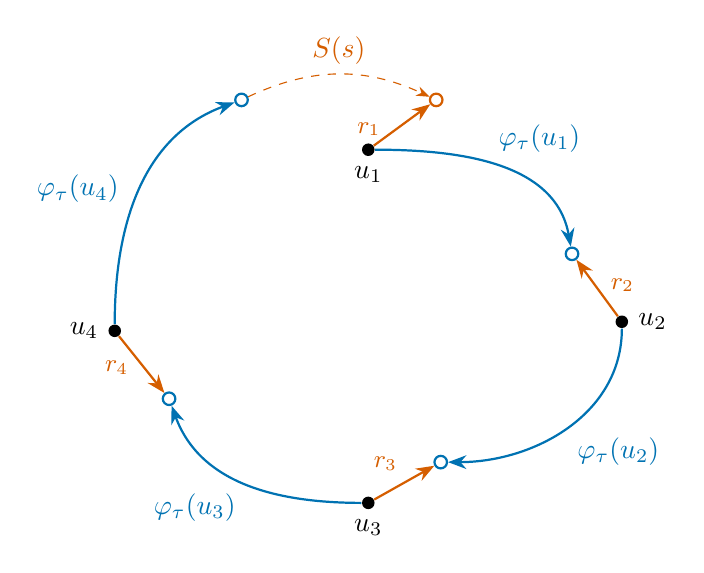
\begin{tikzpicture}[>=Stealth, scale=1.15,
      seed/.style={circle, fill=black, inner sep=1.6pt},
      end/.style={circle, draw=c1, fill=white, inner sep=1.6pt, thick}]
    % seeds
    \node[seed, label=below:{$u_1$}]      (u1) at (0, 2.0) {};
    \node[seed, label=right:{$u_2$}]      (u2) at (2.8, 0.1) {};
    \node[seed, label=below:{$u_3$}]      (u3) at (0, -1.9) {};
    \node[seed, label=left:{$u_4$}]       (u4) at (-2.8, 0.0) {};
    % ends of the segments
    \node[end] (e1) at (2.25, 0.85) {};
    \node[end] (e2) at (0.8, -1.45) {};
    \node[end] (e3) at (-2.2, -0.75) {};
    \node[end] (e4) at (-1.4, 2.55) {};
    \node[end, draw=cr] (w) at (0.75, 2.55) {};
    % segments
    \draw[->, c1, thick] (u1) to[out=0, in=100] node[pos=0.45, above right] {$\varphi_\tau(u_1)$} (e1);
    \draw[->, c1, thick] (u2) to[out=-90, in=0] node[pos=0.5, below right] {$\varphi_\tau(u_2)$} (e2);
    \draw[->, c1, thick] (u3) to[out=180, in=-70] node[pos=0.5, below left] {$\varphi_\tau(u_3)$} (e3);
    \draw[->, c1, thick] (u4) to[out=90, in=200] node[pos=0.5, left=4pt] {$\varphi_\tau(u_4)$} (e4);
    % shift of the last end
    \draw[->, cr, dashed] (e4) to[out=25, in=155] node[above] {$S(s)$} (w);
    % residuals
    \draw[->, cr, thick] (u2) -- (e1) node[pos=0.55, right=2pt] {\small $r_2$};
    \draw[->, cr, thick] (u3) -- (e2) node[pos=0.55, above left=0pt] {\small $r_3$};
    \draw[->, cr, thick] (u4) -- (e3) node[pos=0.55, left=2pt] {\small $r_4$};
    \draw[->, cr, thick] (u1) -- (w)  node[pos=0.4, left=2pt] {\small $r_1$};
  \end{tikzpicture}
  \caption{The loop of multiple shooting with $m = 4$ segments. Each seed $u_i$ (black) is
  advanced by $\tau = T/m$ to the end of its segment (open circles), and the end of the last
  segment is shifted by $S(s)$. The residual $r_{i+1}$ is the gap between the end of segment $i$
  and the next seed, and $r_1$ closes the loop.}
  \label{fig:loop}
\end{figure}

The code holds $z$ in a \code{MultiVector}, with the seeds in a batch \code{X} (section
\ref{sec:batches}) and the scalars in a vector $d = (T, s_1, \dots, s_c)$, read by \code{period},
\code{shift} and \code{nshifts}. The space $\Z$ has the inner product
\begin{equation}
  \ip{z}{w} = \sum_{i=1}^m \ip{u_i}{v_i} + \sum_{j=1}^{1+c} d_j d'_j ,
  \label{eq:ipz}
\end{equation}
for $z$ with seeds $u_i$ and scalars $d$, and $w$ with seeds $v_i$ and scalars $d'$. No weight
balances the seeds against the scalars. The norm thus mixes the states and the period as they
come, and the Krylov method and its trust region inherit this choice.

A Krylov method needs from $\Z$ only linear combinations and inner products. The linear
combinations reach the arrays through broadcasting. An expression such as $w \leftarrow \alpha z +
\beta w$ is split into one broadcast on the seeds and one on the scalars, each in place. On the
seeds it runs on the whole array at once, on whatever device the array lives, or state by state.
The two layouts of the seeds are the subject of the next section.

\section{Batches of states and the propagator}
\label{sec:batches}

The package never advances one state at a time on its own initiative. It hands the propagator a
batch, a collection of $m$ states, so that the propagator can advance them all at once, on threads
or on a GPU, or one after the other. A batch comes in one of two layouts, sketched in
figure~\ref{fig:batches}. In the batched layout it is one array of numbers whose last dimension
runs over the states, such as an $n \times m$ matrix for vectors or an $N_x \times N_y \times m$
array for fields on a grid. In the sliced layout it is a vector of $m$ arrays, one per state, of
any shape. The code dispatches on the two, under the names \code{Batched} and \code{Sliced}.

\begin{figure}
  \centering
  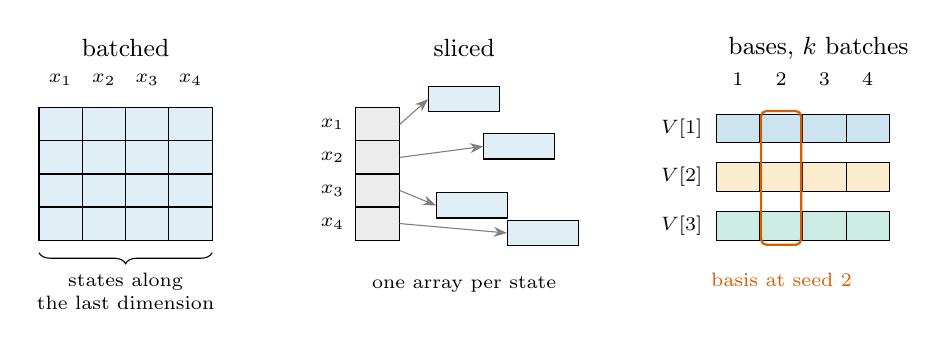
\begin{tikzpicture}[>=Stealth, cell/.style={draw, minimum width=0.55cm, minimum height=0.42cm,
      inner sep=0pt, font=\scriptsize}]
    % ---- batched ----
    \node[font=\small] at (1.1, 2.55) {batched};
    \foreach \j in {1,...,4} {
      \foreach \r in {1,...,4} {
        \node[cell, fill=c1!12] at ({0.55*(\j-1) + 0.275}, {2.0 - 0.42*\r}) {};
      }
      \node[font=\scriptsize] at ({0.55*(\j-1) + 0.275}, 2.15) {$x_\j$};
    }
    \draw[decorate, decoration={brace, mirror, amplitude=4pt}] (0, -0.05) -- (2.2, -0.05)
      node[midway, below=4pt, font=\scriptsize, align=center] {states along\\the last dimension};
    % ---- sliced ----
    \begin{scope}[xshift=4.0cm]
      \node[font=\small] at (1.4, 2.55) {sliced};
      \foreach \j in {1,...,4} {
        \node[cell, fill=gray!15] (p\j) at (0.3, {2.0 - 0.42*\j}) {};
        \node[font=\scriptsize, anchor=east] at (0.0, {2.0 - 0.42*\j}) {$x_\j$};
      }
      \foreach \j/\x/\y in {1/1.4/1.9, 2/2.1/1.3, 3/1.5/0.55, 4/2.4/0.2} {
        \node[cell, fill=c1!12, minimum height=0.32cm, minimum width=0.9cm] (a\j) at (\x, \y) {};
        \draw[->, gray] (p\j.east) -- (a\j.west);
      }
      \node[font=\scriptsize, align=center] at (1.4, -0.45) {one array per state};
    \end{scope}
    % ---- bases ----
    \begin{scope}[xshift=8.6cm]
      \node[font=\small] at (1.3, 2.55) {bases, $k$ batches};
      \foreach \a/\c in {1/c1, 2/c2, 3/c3} {
        \foreach \j in {1,...,4} {
          \node[cell, fill=\c!20, minimum height=0.36cm] at ({0.55*(\j-1) + 0.275}, {2.15 - 0.62*\a}) {};
        }
        \node[font=\scriptsize, anchor=east] at (-0.05, {2.15 - 0.62*\a}) {$V[\a]$};
      }
      \draw[thick, cr, rounded corners=2pt] (0.55*1 + 0.02, 0.05) rectangle (0.55*2 - 0.02, 1.75);
      \node[font=\scriptsize, cr, align=center] at (0.83, -0.4) {basis at seed 2};
      \foreach \j in {1,...,4} {
        \node[font=\scriptsize] at ({0.55*(\j-1) + 0.275}, 2.15) {$\j$};
      }
    \end{scope}
  \end{tikzpicture}
  \caption{The two layouts of a batch of $m = 4$ states, and the bases of the subspace iteration
  (section~\ref{sec:subspace}). Batched, the states are the slices of one array along its last
  dimension. Sliced, each state is an array of its own. The bases are $k$ batches like the
  seeds, one per direction, and the basis at a seed gathers that seed from every batch.}
  \label{fig:batches}
\end{figure}

A propagator is a type of the user's, for which five functions are defined on batches, and a
sixth for the sensitivity of section~\ref{sec:sensitivity}. With
$X = (x_1, \dots, x_m)$ and $V = (v_1, \dots, v_m)$ two batches, they act state by state as
\begin{equation}
  \begin{aligned}
    &\code{propagate!(P, X, $\tau$)} &\qquad x_i &\leftarrow \varphi_\tau(x_i), \\
    &\code{rhs!(P, F, X)}            &\qquad F_i &\leftarrow f(x_i), \\
    &\code{tangent!(P, X, V, $\tau$)} &\qquad x_i &\leftarrow \varphi_\tau(x_i), \quad
      v_i \leftarrow D\varphi_\tau(x_i)\, v_i, \\
    &\code{shift!(P, X, s)}          &\qquad x_i &\leftarrow S(s)\, x_i, \\
    &\code{dshift!(P, G, X, j)}      &\qquad G_i &\leftarrow g_j(x_i), \\
    &\code{forced!(P, X, V, $\tau$)} &\qquad x_i &\leftarrow \varphi_\tau(x_i), \quad
      v_i \leftarrow y_i(\tau).
  \end{aligned}
\end{equation}
Here $y_i(t)$ solves the tangent equation forced by the derivative of $f$ in the parameter,
defined in section~\ref{sec:sensitivity}, from $y_i(0) = v_i$. The functions \code{shift!} and
\code{dshift!} are needed for relative periodic orbits only, and \code{forced!} for the
sensitivity only. In \code{tangent!} the vector $v_i$ is
advanced along the state $x_i$ with the same index, and the states are advanced with the vectors,
since the tangent equation needs them. In practice $\varphi_\tau$ is a numerical scheme with time
steps, and $D\varphi_\tau$ either the derivative of the scheme or a discretisation of the tangent
equation. In both test problems of section~\ref{sec:tests} it is the derivative of the scheme, so
that the tangent map is exact for the discrete map.

\section{The residual}
\label{sec:residual}

The equations of multiple shooting state that each segment ends on the next seed and that the
shifted end of the last segment returns to the first,
\begin{equation}
  \varphi_\tau(u_i) - u_{i+1} = 0, \quad i = 1, \dots, m-1, \qquad
  S(s)\,\varphi_\tau(u_m) - u_1 = 0 .
\end{equation}
The code places the equation of segment $i$ in the row of segment $i+1$, and the closing equation
in row 1. The residual is then
\begin{equation}
  r_{i+1} = \varphi_\tau(u_i) - u_{i+1}, \qquad r_1 = S(s)\,\varphi_\tau(u_m) - u_1,
  \label{eq:residual}
\end{equation}
with a zero scalar part, since the phase conditions act on the Newton step only
(section~\ref{sec:jacobian}). Three operators on $\X^m$ write this compactly. Let
$\Phi_\tau(X) = (\varphi_\tau(x_1), \dots, \varphi_\tau(x_m))$ advance every state, let
$\Sigma_s(X) = (x_1, \dots, x_{m-1}, S(s)x_m)$ shift the last one, and let the roll
\begin{equation}
  \roll(x_1, x_2, \dots, x_m) = (x_m, x_1, \dots, x_{m-1})
\end{equation}
move every state forward by one slot, cyclically. The residual is
\begin{equation}
  F(z) = \big(\roll\, \Sigma_s \Phi_\tau(U) - U,\; 0\big), \qquad U = (u_1, \dots, u_m).
  \label{eq:F}
\end{equation}

The reordering has two purposes. It makes the Jacobian minus the identity plus a cyclic block
subdiagonal (section~\ref{sec:jacobian}), and it lets the residual be computed in place in a
single batch. \code{Residual(P)} called as \code{F(r, z)} follows \eqref{eq:F} from right to left,
\begin{equation}
  r \leftarrow z, \qquad
  r_i \leftarrow \varphi_\tau(r_i), \qquad
  r_m \leftarrow S(s)\, r_m, \qquad
  r \leftarrow \roll\, r, \qquad
  r \leftarrow r - z ,
\end{equation}
with $r$ the only storage. A call integrates all the seeds once over $\tau$, in one call of
\code{propagate!}.

The roll is the only step that moves states between slots, and it must not need a second batch,
since a batch may fill a large part of the memory of a GPU. In the batched layout the code rolls
by two reversals along the last dimension, first of all the slots and then of the slots $2$ to
$m$. After the first reversal slot $i$ holds $x_{m+1-i}$. The second maps slot $i \geq 2$ to slot
$m + 2 - i$, which held $x_{m+1-(m+2-i)} = x_{i-1}$, and leaves $x_m$ in slot 1. The result is
$\roll X$, as figure~\ref{fig:roll} shows. A reversal swaps pairs of entries in place, so that the roll
needs no second batch and moves every entry twice. In the sliced layout
the roll permutes the references to the states, and moves no data at all.

\begin{figure}
  \centering
  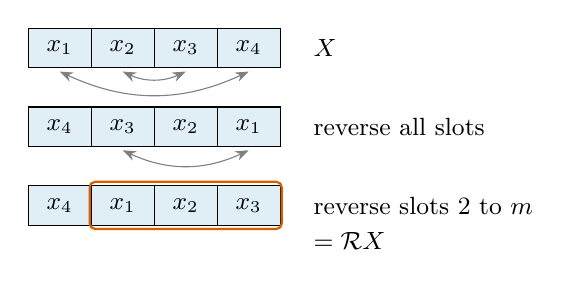
\begin{tikzpicture}[>=Stealth, box/.style={draw, minimum width=0.8cm, minimum height=0.5cm,
      fill=c1!12, font=\small}]
    \foreach \row/\a/\b/\c/\d/\lab in {0/x_1/x_2/x_3/x_4/{$X$},
                                      1/x_4/x_3/x_2/x_1/{reverse all slots},
                                      2/x_4/x_1/x_2/x_3/{reverse slots $2$ to $m$}} {
      \node[box] at (0, -1.0*\row) {$\a$};
      \node[box] at (0.8, -1.0*\row) {$\b$};
      \node[box] at (1.6, -1.0*\row) {$\c$};
      \node[box] at (2.4, -1.0*\row) {$\d$};
      \node[anchor=west, font=\small] at (3.1, -1.0*\row) {\lab};
    }
    \draw[<->, gray] (0, -0.3) to[bend right=25] (2.4, -0.3);
    \draw[<->, gray] (0.8, -0.3) to[bend right=25] (1.6, -0.3);
    \draw[<->, gray] (0.8, -1.3) to[bend right=25] (2.4, -1.3);
    \draw[thick, cr, rounded corners=2pt] (0.38, -2.3) rectangle (2.82, -1.7);
    \node[anchor=west, font=\small] at (3.1, -2.45) {$= \roll X$};
  \end{tikzpicture}
  \caption{The roll in place, by two reversals along the last dimension. The second reversal acts
  on the slots $2$ to $m$ (frame). Each state ends in the slot after its own, and the last in slot
  1.}
  \label{fig:roll}
\end{figure}

\section{The Jacobian}
\label{sec:jacobian}

We differentiate $F$ at $z$ along $v = (v_1, \dots, v_m, \delta T, \delta s_1, \dots, \delta
s_c)$. Let $\psi_i = D\varphi_\tau(u_i)$ be the tangent map of segment $i$, and let $\delta\tau =
\delta T / m$ be the change of the length of a segment. Since $\partial_\tau \varphi_\tau(u) =
f(\varphi_\tau(u))$, the row of segment $i + 1$ is
\begin{equation}
  (Jv)_{i+1} = \psi_i v_i - v_{i+1} + \delta\tau\, f(\varphi_\tau(u_i)), \qquad i = 1, \dots, m-1 .
\end{equation}
Row 1 holds the shifted end of the last segment,
\begin{equation}
  w = S(s)\,\varphi_\tau(u_m) .
\end{equation}
Its derivative with respect to $T$ is $S(s) f(\varphi_\tau(u_m))/m$, which by equivariance equals
$f(w)/m$, and its derivative with respect to $s_j$ is $g_j(w)$ by the identity of
section~\ref{sec:setting}. Hence
\begin{equation}
  (Jv)_1 = S(s)\psi_m v_m - v_1 + \delta\tau\, f(w) + \sum_{j=1}^c \delta s_j\, g_j(w).
\end{equation}
The code evaluates $f$ and the generators at the shifted end, rather than shifting $f$, which the
equivariance allows.

The scalar rows hold the phase conditions. At a solution the seed part of $J$ has the null
directions
\begin{equation}
  (f(u_1), \dots, f(u_m), 0, 0), \qquad (g_j(u_1), \dots, g_j(u_m), 0, 0), \quad j = 1, \dots, c .
\end{equation}
Indeed $\psi_i f(u_i) = f(\varphi_\tau(u_i)) = f(u_{i+1})$ by \eqref{eq:neutral}, and in row 1
$S(s)\psi_m f(u_m) = f(S(s)\varphi_\tau(u_m)) = f(u_1)$. The same holds for $g_j$, since $T_j$
commutes with $S(s)$. These directions move the solution along the family of section
\ref{sec:setting}. The scalar rows
\begin{equation}
  (Jv)_{T} = \ip{f(u_1)}{v_1}, \qquad (Jv)_{s_j} = \ip{g_j(u_1)}{v_1},
\end{equation}
exclude them, so that the Newton step is orthogonal at the first seed to the time derivative and
to the generators. These are the phase conditions. They fix the phase of the first seed of the
step rather than of the point, which is why the scalar part of the residual is zero. With them $J$
is square, with $mn + 1 + c$ rows and columns. Figure~\ref{fig:jacobian} shows its blocks, minus
the identity on the diagonal, the tangent maps on the cyclic subdiagonal, and the extra columns
and rows.

\begin{figure}
  \centering
  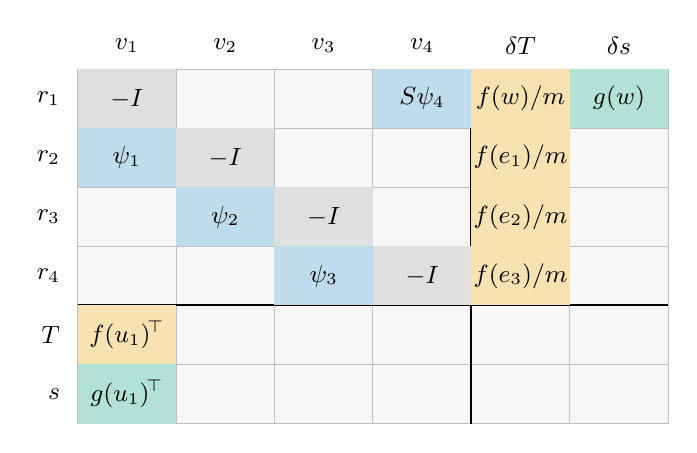
\begin{tikzpicture}[cell/.style={minimum width=1.25cm, minimum height=0.75cm, inner sep=0pt,
      font=\small}]
    \def\w{1.25}
    \def\h{0.75}
    % frame and grid
    \fill[gray!6] (0, 0) rectangle (6*\w, -6*\h);
    \draw[gray!50] (0, 0) grid[xstep=\w, ystep=\h] (6*\w, -6*\h);
    \draw[thick] (4*\w, 0) -- (4*\w, -6*\h);
    \draw[thick] (0, -4*\h) -- (6*\w, -4*\h);
    % blocks
    \newcommand{\blk}[4]{\fill[#4] ({(#2-1)*\w}, {-(#1-1)*\h}) rectangle ({#2*\w}, {-#1*\h});
      \node[cell] at ({(#2-0.5)*\w}, {-(#1-0.5)*\h}) {#3};}
    \blk{1}{1}{$-I$}{gray!25}
    \blk{2}{2}{$-I$}{gray!25}
    \blk{3}{3}{$-I$}{gray!25}
    \blk{4}{4}{$-I$}{gray!25}
    \blk{2}{1}{$\psi_1$}{c1!25}
    \blk{3}{2}{$\psi_2$}{c1!25}
    \blk{4}{3}{$\psi_3$}{c1!25}
    \blk{1}{4}{$S\psi_4$}{c1!25}
    \blk{1}{5}{$f(w)/m$}{c2!30}
    \blk{2}{5}{$f(e_1)/m$}{c2!30}
    \blk{3}{5}{$f(e_2)/m$}{c2!30}
    \blk{4}{5}{$f(e_3)/m$}{c2!30}
    \blk{1}{6}{$g(w)$}{c3!30}
    \blk{5}{1}{$f(u_1)^{\!\top}$}{c2!30}
    \blk{6}{1}{$g(u_1)^{\!\top}$}{c3!30}
    % labels
    \foreach \j/\l in {1/v_1, 2/v_2, 3/v_3, 4/v_4, 5/\delta T, 6/\delta s} {
      \node[font=\small] at ({(\j-0.5)*\w}, 0.3) {$\l$};
    }
    \foreach \i/\l in {1/r_1, 2/r_2, 3/r_3, 4/r_4, 5/T, 6/s} {
      \node[font=\small, anchor=east] at (-0.1, {-(\i-0.5)*\h}) {$\l$};
    }
  \end{tikzpicture}
  \caption{The blocks of the Jacobian for $m = 4$ segments and one shift, with $S = S(s)$, $e_i =
  \varphi_\tau(u_i)$ the end of segment $i$ and $w = S(s)\,e_4$. Rows follow the residual \eqref{eq:residual}, columns the unknowns. Blank
  blocks are zero. The last two rows hold the phase conditions.}
  \label{fig:jacobian}
\end{figure}

The code never forms these blocks. \code{mul!(out, J, v)} follows the residual step by step, with
the seeds advanced again together with the vector,
\begin{equation}
  \text{out} = \Big(\roll\,\big(\Sigma_s \Psi V + \delta\tau\, F_{\mathrm{e}} + E_m \textstyle\sum_j \delta s_j\, G_j\big) - V,\;
    \ip{f(u_1)}{v_1},\; \ip{g_j(u_1)}{v_1}\Big),
\end{equation}
where $\Psi V = (\psi_1 v_1, \dots, \psi_m v_m)$ comes from one call of \code{tangent!} along a copy
of the seeds, $F_{\mathrm{e}} = (f(\varphi_\tau(u_1)), \dots, f(\varphi_\tau(u_{m-1})), f(w))$
holds the time derivative at the ends of the segments, the last shifted, $G_j = g_j(w)$, and $E_m$
places a state in the last slot. The ends of the segments do not depend on $v$. \code{update!(J,
z)} computes $F_{\mathrm{e}}$, the $G_j$, $f(u_1)$ and $g_j(u_1)$ when $J$ moves to a new point,
with one integration of the seeds, and keeps $z$ itself rather than a copy. Each product then
integrates the seeds once more with the vector, so that it costs one tangent integration of all
the segments over $\tau$, or a time $T$ integrated in all. This avoids storing the trajectory of
every segment, at the price of the nonlinear part of the integration in every product.

One remark is in order on the column of the period. The tangent maps are those of the numerical
scheme, but the column of the period uses $f$ of the continuous system. The derivative of the
discrete map with respect to its length differs from $f$ at the end point by a quantity of the
order of the error of the scheme. The Jacobian is thus exact for the discrete residual in every
column but that of the period, where it carries this error. We return to its effect on the
Newton iterations in section~\ref{sec:tests}.

\section{Newton--Krylov iterations}
\label{sec:newton}

The equations $F(z) = 0$ are solved by \code{nkroot!(F, J, z)} of \code{NKRoots.jl}, which
overwrites $z$ with the solution. At every iteration it calls \code{update!(J, z, r)}, which moves
the Jacobian to the current point and ignores the residual $r$. The residual is used only by
Jacobians that approximate the products by finite differences, for which \code{NKRoots.jl} defines
the same function. The Arnoldi iteration started from $-r$ then builds an orthonormal basis of a
Krylov space of $J$, with the inner product \eqref{eq:ipz}, and the step minimises the norm of the
linear model $r + J\delta$ over that space, subject to a trust region $\|\delta\| \leq \Delta$. A
step inside the trust region is the GMRES step. A step on its boundary is a hookstep, which
damps the directions of small singular values of the small Hessenberg matrix. The radius grows or
shrinks with the ratio of the actual to the predicted reduction of $\|r\|^2$. The Krylov space
grows until the GMRES residual falls below a tolerance or reaches a largest dimension, and every
new direction costs one product with $J$, hence one tangent integration of the seeds.

\section{Sensitivity to a parameter}
\label{sec:sensitivity}

Let the right-hand side depend on a parameter $p$, $f(u; p)$, and let $z(p)$ be a family of
orbits, so that $F(z(p), p) = 0$. Differentiating in $p$ gives the linear system
\begin{equation}
  J\, \frac{dz}{dp} = -\frac{\partial F}{\partial p},
  \label{eq:sensitivity}
\end{equation}
with $J$ the Jacobian of section~\ref{sec:jacobian} at the orbit. Its right-hand side follows the
residual. The end of segment $i$ depends on $p$ through the flow, and its derivative $y_i(\tau) =
\partial \varphi_\tau(u_i) / \partial p$ solves the tangent equation forced by the derivative of
$f$ in $p$,
\begin{equation}
  \dot y = \frac{\partial f}{\partial u}(\varphi_t(u_i))\, y + \frac{\partial f}{\partial p}(\varphi_t(u_i)),
  \qquad y(0) = 0 .
\end{equation}
The shift does not depend on $p$, and neither do the phase conditions, so that with $Y = (y_1(\tau),
\dots, y_m(\tau))$
\begin{equation}
  -\frac{\partial F}{\partial p} = \big(-\roll\, \Sigma_s Y,\; 0\big).
\end{equation}
\code{tangent\_sensitivity(P, z)} builds the Jacobian at the converged orbit $z$ itself, with one
integration of the seeds. The Jacobian of the Newton iterations would not do, since it was last
moved to the iterate before the converged one. The right-hand side is built as the residual is.
The seeds are copied into the work batch, the vectors set to zero, both advanced with
\code{forced!}, the last slot shifted, the batch rolled and the sign changed, for one forced
integration of the seeds.

The code solves \eqref{eq:sensitivity} by its own GMRES, from zero and without restarts. The
Arnoldi basis of the Krylov space is orthonormalised by modified Gram--Schmidt, twice, in the
inner product \eqref{eq:ipz}, and Givens rotations reduce the Hessenberg matrix to triangular form
as the basis grows, which gives the norm of the residual at every iteration at no cost. The
iteration stops when this norm falls below a relative tolerance, or when the basis reaches its
largest size, with one product with $J$ per iteration. The scalar part of the solution holds
$dT/dp$ and the derivatives of the shifts.
The phase rows make the derivative of the first seed orthogonal to $f(u_1)$ and to the
generators at $z$, which picks one derivative of the seeds among those that differ by a move
along the family of section~\ref{sec:setting}. The derivatives of the period and of the shifts do
not depend on this choice, since a move along the family changes neither. As for the Newton iterations, the column of
the period carries the error of the scheme into the solution.

In the Lorenz test the parameter is $\rho$, with $\partial f/\partial\rho = (0, x_1, 0)$, and the
forced tangent is advanced by the stages of the scheme linearised with the forcing, the derivative
of the scheme in $\rho$. For the orbit AB at $\rho = 28$ it gives $dT/d\rho \approx -0.0393$, which
agrees with central differences of the period of the orbit converged at $\rho = 28 \pm 10^{-4}$
within the relative tolerance $10^{-6}$ of the test.

\section{Subspace iteration along the loop}
\label{sec:subspace}

The tangent maps along the loop stretch a few directions, keep the time derivative and the
generators, and contract the rest. A preconditioner for the Newton system may act exactly on the
first two groups, and to that end the package computes them by subspace iteration along the loop.
This section describes the iteration on a fixed loop, the point $z$ of a Jacobian.

Let $\tilde\psi_m = S(s)\psi_m$. Going once round the loop from seed $i$ gives the cyclic monodromy
\begin{equation}
  M_i = \psi_{i-1} \cdots \psi_1\, \tilde\psi_m\, \psi_{m-1} \cdots \psi_i ,
\end{equation}
and $M_1 = \tilde\psi_m \psi_{m-1}\cdots\psi_1$ is the tangent map of the whole loop seen from the
first seed. On a periodic orbit $M_1$ is the monodromy matrix, and on a relative one its product
with the shift. Since $\psi_i M_i = M_{i+1} \psi_i$, the cyclic monodromies share their nonzero
eigenvalues, the Floquet multipliers $\Lambda_1, \Lambda_2, \dots$, which we order by decreasing
modulus. We write $\lambda_j = \log|\Lambda_j| / T$ for the Floquet exponents.

The package keeps at every seed $i$ an orthonormal basis $V_i$ of $k$ directions, random at the
start. A subspace step, \code{iterate!}, carries every basis over its segment and orthonormalises
it at the seed it reaches,
\begin{equation}
  V_{i+1} \leftarrow \mathrm{orth}(\psi_i V_i), \quad i = 1, \dots, m-1, \qquad
  V_1 \leftarrow \mathrm{orth}(\tilde\psi_m V_m),
  \label{eq:step}
\end{equation}
all the seeds at once, as figure~\ref{fig:subspace} sketches. After $r$ steps the basis at seed $i$
spans the image of the starting basis at seed $i - r$, modulo $m$, by the $r$ tangent maps in
between. For $r = qm$ it spans $M_i^q V_i^{(0)}$, so that every seed runs the simple subspace
iteration of \citet[algorithm 5.1]{saad2011} with its own cyclic monodromy. For each eigenvector
$x_j$ of $M_i$ among the $k$ dominant ones, \citet[theorem 5.2]{saad2011} bounds the distance from
the span after $q$ powers by a constant times $|\Lambda_{k+1}/\Lambda_j|^q$, up to a term that
vanishes as $q$ grows. In the exponents, and per step,
\begin{equation}
  \varepsilon_j(r) \sim e^{-(\lambda_j - \lambda_{k+1})\, r\tau}, \qquad r = qm ,
  \label{eq:rate}
\end{equation}
a rate that holds on average between multiples of $m$. The larger $k$, the further the gap
$\lambda_j - \lambda_{k+1}$, and the fewer the steps.

\begin{figure}
  \centering
  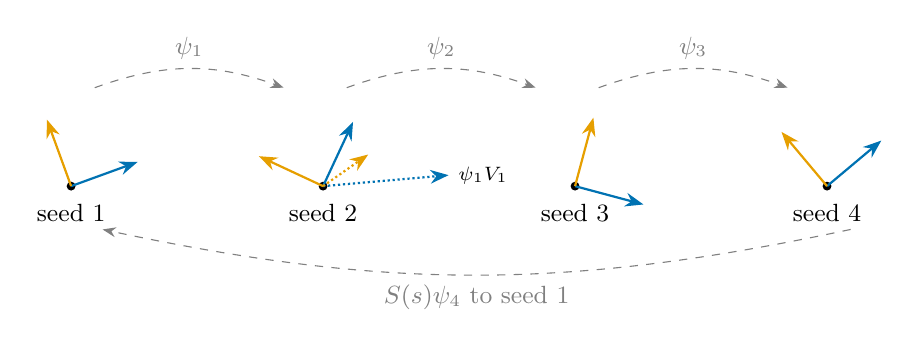
\begin{tikzpicture}[>=Stealth, scale=1.0]
    % seeds on a line
    \foreach \i in {1,...,4} {
      \coordinate (s\i) at ({3.2*(\i-1)}, 0);
      \fill (s\i) circle (1.6pt);
      \node[below=3pt, font=\small] at (s\i) {seed \i};
    }
    % orthonormal frames at every seed, before the step
    \foreach \i/\ang in {1/20, 2/65, 3/-15, 4/40} {
      \draw[->, c1, thick] (s\i) -- ++(\ang:0.9);
      \draw[->, c2, thick] (s\i) -- ++(\ang+90:0.9);
    }
    % the image of the frame of seed 1 at seed 2, and its orthonormalisation
    \draw[->, gray, dashed] ($(s1)+(0.3,1.25)$) to[bend left=20] node[above, font=\small] {$\psi_1$} ($(s2)+(-0.5,1.25)$);
    \draw[->, gray, dashed] ($(s2)+(0.3,1.25)$) to[bend left=20] node[above, font=\small] {$\psi_2$} ($(s3)+(-0.5,1.25)$);
    \draw[->, gray, dashed] ($(s3)+(0.3,1.25)$) to[bend left=20] node[above, font=\small] {$\psi_3$} ($(s4)+(-0.5,1.25)$);
    \draw[->, gray, dashed] ($(s4)+(0.3,-0.55)$) to[bend left=12] node[below, font=\small] {$S(s)\psi_4$ to seed 1} ($(s1)+(0.4,-0.55)$);
    % image at seed 2, skewed and stretched
    \draw[->, c1, densely dotted, thick] (s2) -- ++(5:1.6);
    \draw[->, c2, densely dotted, thick] (s2) -- ++(35:0.7);
    \node[font=\scriptsize, anchor=west] at ($(s2)+(5:1.6)$) {$\psi_1 V_1$};
  \end{tikzpicture}
  \caption{A subspace step with $k = 2$. Every frame is carried over its segment, the last shifted
  back to the first seed, and orthonormalised where it lands, all seeds at once. At seed 2 the
  dotted frame is the image of the frame of seed 1, which the step replaces by an orthonormal
  basis of its span, the first direction kept.}
  \label{fig:subspace}
\end{figure}

The step treats all seeds at once, which is how the products of the Jacobian treat them, and this
has a price in time integrated. In the algorithm of \citet[algorithm 6.2]{lust1997} one sweep
carries a single basis from the first seed through all the segments in turn, so that it advances
the basis by a whole loop for $k$ integrations of time $T$. A step of \eqref{eq:step} also
integrates $k$ directions over every segment, but advances each basis by one segment only. For
the same accuracy it thus integrates $m$ times longer in all. In exchange all segments are
integrated at once, so that on a batch that advances the $m$ segments in the wall time of one,
the two reach the same accuracy in the same wall time.

The bases are stored as $k$ batches like the seeds, one per direction. Batch $V[a]$ holds
direction $a$ at every seed, $V[a] = (v_1^a, \dots, v_m^a)$, and the basis at seed $i$ gathers
slot $i$ of every batch (figure~\ref{fig:batches}). Each batch is then carried exactly as a vector
of the Jacobian. For each direction $a$ the seeds are copied into a work batch,
\code{tangent!} advances them with $V[a]$, the last slot is shifted and the batch is rolled. A step
thus costs $k$ tangent integrations of the seeds, a time $kT$ integrated, with no function of the
propagator beyond those of section~\ref{sec:batches}.

The orthonormalisation is the modified Gram--Schmidt process across the batches, seed by seed. In
the order of the directions,
\begin{equation}
  v_i^a \leftarrow v_i^a - \ip{v_i^b}{v_i^a}\, v_i^b, \quad b = 1, \dots, a - 1, \qquad
  v_i^a \leftarrow v_i^a / \|v_i^a\|,
\end{equation}
at every seed $i$, with one coefficient per seed, and the whole process runs twice so that the
bases stay orthogonal to rounding. The coefficients are inner products state by state, which the
code computes for all seeds at once and broadcasts back against the batches, in either layout.
Gram--Schmidt in order is triangular. The first $p$ directions after a step span the images of the
first $p$ before it, for every $p \leq k$, and the first $p$ directions run a subspace iteration of
dimension $p$ of their own. This is the observation behind the proof of \citet[theorem
5.1]{saad2011}, extended there to the first $j$ columns. Without a projection step, the additional
$k - p$ directions do not speed up the first $p$ columns themselves, whose span converges at the
slower rate of an iteration of dimension $p$, the rate \eqref{eq:rate} with $j = k = p$. The
measure of the next section tests these $p$ directions, and so follows this rate.

\section{The accuracy of the bases}
\label{sec:accuracy}

To decide when the bases are accurate enough, we follow \citet[sections 2.4.4 and
6.3.3]{lust1997}, in the letters of the code. For a single shooting, with $U$ the first $k$ ordered
Schur vectors and $V = MU$ their images, he measures
\begin{equation}
  \varepsilon_k = \max_{\|p\| = 1} \big\| (I - UU^{\!\top}) M U p \big\| ,
\end{equation}
the largest singular value of $Z = (I - UU^{\!\top}) V$, the part of the image of the subspace that
falls outside it. It vanishes when the span of $U$ is invariant. It costs no further products with
$M$, since $Z^{\!\top} Z = V^{\!\top} V - (U^{\!\top} V)^{\!\top} (U^{\!\top} V)$ involves $k \times k$
matrices only.

Here the bases before a step are $U_i$, orthonormal $n \times k$ at every seed. After the tangent
maps, the shift and the roll, slot $i$ holds the image of the basis of the seed before,
\begin{equation}
  V_i = \psi_{i-1} U_{i-1}, \quad i = 2, \dots, m, \qquad V_1 = \tilde\psi_m U_m ,
\end{equation}
and \code{iterate!}, before it orthonormalises, forms the remainders of all $k$ directions,
$Z_i = V_i - U_i (U_i^{\!\top} V_i) = (I - U_iU_i^{\!\top}) V_i$, and keeps the $k \times k$ matrices
$Z_i^{\!\top} Z_i$ and $U_i^{\!\top} V_i$, from the inner products between the batches, one per seed,
brought to the host. For the first $p$ directions, with $E_p$ the first $p$ columns of the
identity, $U_i^p = U_i E_p$ and $V_i^p = V_i E_p$, the remainder is that of all $k$ plus its part
along the other $k - p$ directions, two parts orthogonal to each other, so that
\begin{equation}
  Z_i^p = \big(I - U_i^p U_i^{p\top}\big) V_i^p, \qquad
  Z_i^{p\top} Z_i^p = \big(Z_i^{\!\top} Z_i\big)_{1:p,\,1:p}
                    + \big(U_i^{\!\top} V_i\big)_{p+1:k,\,1:p}^{\!\top} \big(U_i^{\!\top} V_i\big)_{p+1:k,\,1:p} ,
\end{equation}
a sum of two positive semidefinite blocks of the matrices kept, and \code{change(S; p)} returns
\begin{equation}
  \varepsilon_p = \max_i \sigma_{\max}\big(Z_i^p\big)
                = \max_i \sqrt{\lambda_{\max}\big(Z_i^{p\top} Z_i^p\big)} .
\end{equation}
Figure~\ref{fig:lust} shows the geometry at one seed. With $p$ the number of unstable and neutral
directions it measures the error of these directions.

\begin{figure}
  \centering
  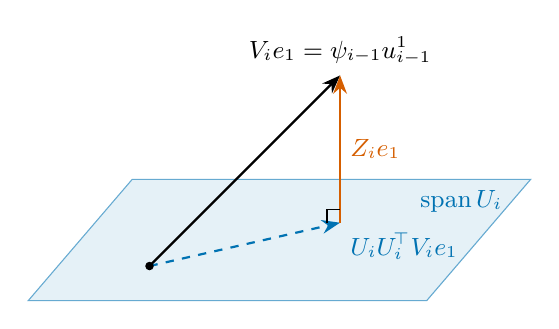
\begin{tikzpicture}[>=Stealth, scale=1.1]
    % the plane span U_i
    \fill[c1!10] (0, 0) -- (4.6, 0) -- (5.8, 1.4) -- (1.2, 1.4) -- cycle;
    \draw[c1!60] (0, 0) -- (4.6, 0) -- (5.8, 1.4) -- (1.2, 1.4) -- cycle;
    \node[c1, font=\small] at (5.0, 1.15) {$\mathrm{span}\, U_i$};
    % V, its projection and Z
    \coordinate (o) at (1.4, 0.4);
    \coordinate (p) at (3.6, 0.9);
    \coordinate (w) at (3.6, 2.6);
    \draw[->, thick] (o) -- (w) node[above, font=\small] {$V_i e_1 = \psi_{i-1} u_{i-1}^1$};
    \draw[->, thick, dashed, c1] (o) -- (p) node[below right, font=\small] {$U_i U_i^{\!\top} V_i e_1$};
    \draw[->, thick, cr] (p) -- (w) node[midway, right, font=\small] {$Z_i e_1$};
    \draw (3.45, 0.9) -- (3.45, 1.05) -- (3.6, 1.05);
    \fill (o) circle (1.4pt);
  \end{tikzpicture}
  \caption{Lust's measure at one seed. The image of a direction of the basis at the seed before
  splits into its projection on the span of the basis here and a remainder $Z_i e_1$, which
  vanishes when the span is invariant. $\varepsilon_p$ is the largest singular value of the
  remainders of the first $p$ directions, the largest over the seeds.}
  \label{fig:lust}
\end{figure}

The measure departs from Lust's in one point, it is taken at every seed. In a sweep of
\citet[algorithm 6.2]{lust1997} the basis at every intermediate seed is by construction the
orthonormalised image of the one before, and only the seed that closes the loop carries a
remainder. Here every seed receives the image of a basis that the step has not yet seen, so that
each has a remainder of its own, and the code takes the largest.

The iteration itself departs from Lust's in its lack of a projection step. In Lust's algorithm a
projection step makes $U^{\!\top} V$ block upper triangular, so that the projections of the image
of the first $p$ directions on these directions and on all $k$ coincide. The first $p$ directions
then gain from the other $k - p$, and their measure falls at the rate \eqref{eq:rate} with
$j = p$, that of an iteration of dimension $k$. The step \eqref{eq:step} has no projection, and by
section~\ref{sec:subspace} the measure follows the slower rate of an iteration of dimension $p$,
whatever $k$ is.

Two limits apply. The first is rounding. Lust forms $Z^{\!\top}Z$ as the difference
$V^{\!\top}V - (U^{\!\top}V)^{\!\top}(U^{\!\top}V)$, which he regards as less stable than a
factorisation of $Z$ but accurate enough for the purpose, and which resolves the measure down to
about $\sqrt{\epsilon}\,\|V\|$ only, with $\epsilon$ the machine precision. The code forms $Z$
itself, so that its Gram matrix carries no cancellation and the measure resolves down to about
$\epsilon\,\|V\|$. The second is that $p$ should not split
a complex pair of multipliers, as Lust also requires. The two directions of a pair rotate into
each other at every step, so that the span of only one of them never settles.

\section{Two test problems}
\label{sec:tests}

The tests run on two systems with propagators written for them. The Lorenz system is small and
has no symmetry, and it checks every piece in both layouts. The Kuramoto--Sivashinsky equation has
a continuous translation symmetry, and it checks the shifts.

\subsection{The Lorenz system}

The Lorenz system at $\sigma = 10$, $\rho = 28$ and $\beta = 8/3$ is advanced by the classical
fourth-order Runge--Kutta scheme, with $\lceil \tau/\Delta t \rceil$ steps of equal length over a
time $\tau$ and $\Delta t = 10^{-3}$. The tangent vectors are advanced by the same stages
linearised along those of the state, so that the tangent map is the derivative of the scheme. The
right-hand side is written for one state, and the same scheme serves a $3 \times m$ matrix,
batched, and a vector of 3-vectors, sliced.

The guess of the shortest orbit, AB, comes from the closest return of a long trajectory with a
period between 1.4 and 1.7, found once offline. Its four seeds lie at a distance of about $0.4$
from closing, and figure~\ref{fig:lorenz} compares them with the converged orbit. The search
converges in five iterations, the first a hookstep, to $T = 1.5586522$ in both layouts, and the
last iterations converge quadratically (figure~\ref{fig:newton}).

\begin{figure}
  \centering
  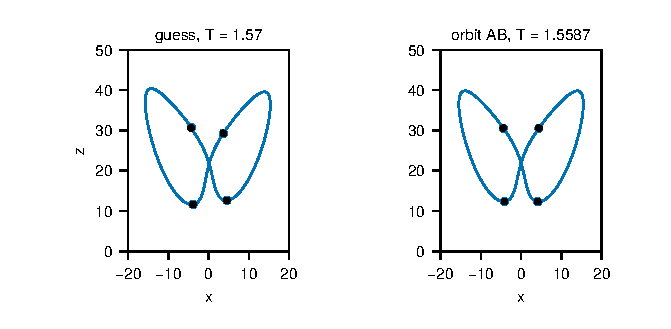
\includegraphics[width=0.85\textwidth]{figures/lorenz.pdf}
  \caption{The guess of the Lorenz orbit AB from the tests (left) and the converged orbit (right),
  in the $(x, z)$ plane. The four seeds are the black dots and the curves their segments. At this
  scale the gaps of the guess are small.}
  \label{fig:lorenz}
\end{figure}

\begin{figure}
  \centering
  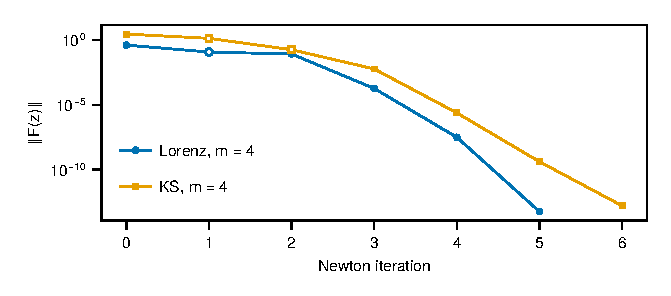
\includegraphics[width=0.8\textwidth]{figures/newton.pdf}
  \caption{The norm of the residual over the Newton iterations of the two searches of the tests.
  Open markers are hooksteps, filled ones GMRES steps inside the trust region.}
  \label{fig:newton}
\end{figure}

On the orbit the dense monodromy, built from the tangent maps of three unit vectors, has the
multipliers $4.7$, $1$ and about $10^{-10}$. With $k = 2$ the bases hold the unstable and the
neutral direction. The gap to the third multiplier is so wide that $\varepsilon_2$ falls by about
three orders of magnitude per step, as \eqref{eq:rate} predicts, down to rounding, near
$10^{-15}$, in seven steps (figure~\ref{fig:subspacedata}, top left). The unstable direction alone is set apart
from the neutral one only by the factor $4.7$ over a loop, so that $\varepsilon_1$ falls by about
$0.7$ per step, on average over a loop, the rate of an iteration of dimension one.

\subsection{The Kuramoto--Sivashinsky equation}

The equation $u_t = -u u_x - u_{xx} - u_{xxxx}$ on $[0, L)$ with periodic boundary conditions and
$L = 22$ has the translations $S(s)u(x) = u(x + s)$, with the generator $g = \partial_x$. A state is
$u$ on $N = 64$ grid points, and a batch is an $N \times m$ matrix with one state per column, so that
the transforms run along the first dimension for the whole batch at once. With the Fourier
coefficients $\hat u_k$ and the wavenumbers $\kappa = 2\pi k / L$ the equation reads
\begin{equation}
  \hat u_t = \Lambda \hat u + \mathcal{N}(\hat u), \qquad \Lambda = \kappa^2 - \kappa^4, \qquad
  \mathcal{N}(\hat u) = -\tfrac{i\kappa}{2}\, \widehat{u^2} .
\end{equation}
Only the modes $1 \leq k < N/3$ are kept. A product of two fields with $|k| < N/3$ has modes $|k| <
2N/3$, and on $N$ points mode $k$ aliases onto $k - N$, which for $N/3 \leq k < 2N/3$ falls outside
the band kept. The kept modes of the product are therefore exact, the truncated system is the
Galerkin truncation, and the shift $\hat u_k \mapsto e^{i\kappa s}\hat u_k$ commutes with it
exactly. The mean, which the flow conserves, is set to zero, as in \citet[equation
(2.4)]{cvitanovic2010}.

The steps are those of the fourth-order exponential Runge--Kutta scheme ETDRK4 of Cox and Matthews,
as written by \citet{kassam2005}. With step $h$ and the mode-wise coefficients $E = e^{h\Lambda}$
and $E_2 = e^{h\Lambda/2}$,
\begin{equation}
  \begin{aligned}
    a &= E_2 \hat v + Q\, \mathcal{N}(\hat v), \qquad
    b = E_2 \hat v + Q\, \mathcal{N}(a), \qquad
    c = E_2 a + Q\, \big(2\mathcal{N}(b) - \mathcal{N}(\hat v)\big), \\
    \hat v &\leftarrow E \hat v + f_1 \mathcal{N}(\hat v) + 2 f_2 \big(\mathcal{N}(a) + \mathcal{N}(b)\big)
      + f_3 \mathcal{N}(c),
  \end{aligned}
\end{equation}
with
\begin{equation}
  \begin{aligned}
    Q &= h\,\frac{e^{z/2} - 1}{z}, &\qquad
    f_1 &= h\,\frac{-4 - z + e^z(4 - 3z + z^2)}{z^3}, \\
    f_2 &= h\,\frac{2 + z + e^z(z - 2)}{z^3}, &\qquad
    f_3 &= h\,\frac{-4 - 3z - z^2 + e^z(4 - z)}{z^3},
  \end{aligned}
\end{equation}
evaluated at $z = h\Lambda$. These functions cancel badly for small $z$, and following
\citet{kassam2005} the code takes each as the mean of the same function over $32$ points on the
upper half of a circle of radius one centred at $h\Lambda$, real part. The tangent vectors are
advanced by the stages linearised along those of the state, with $\mathcal{N}'(\hat v)\delta\hat v =
-i\kappa\, \widehat{u\,\delta u}$, so that the tangent map is again the derivative of the scheme.
Against central differences of the propagator it agreed to about $10^{-9}$, and the shift and the
flow commuted to rounding.

We search for the shortest relative periodic orbit of \citet[figure 6.1(a)]{cvitanovic2010}, with
$T_p = 16.3$ and $\ell_p = 2.86$, which their equation (2.20) defines as $u(x + \ell_p, T_p) = u(x,
0)$, the same condition as \eqref{eq:rpo}. The guess of the tests has four seeds along a trajectory
from a random state, at the closest return up to a shift with a period between 15.8 and 16.8 and a
shift of size between 2 and 4. Without the window on the shift the closest returns were slow passes
near an equilibrium, from which the searches converged to that equilibrium or to a vanishing
period. The search converges in
six iterations, two hooksteps first, to $T = 16.3148$ and $s = -2.8634$ (figure~\ref{fig:ks}). The
sign is that of the symmetric partner $-u(-x)$ of the orbit, which has the opposite shift
\citep[section 2.3]{cvitanovic2010}.

\begin{figure}
  \centering
  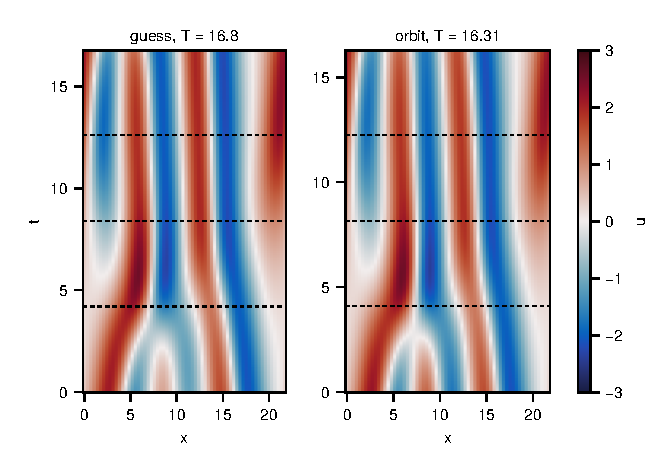
\includegraphics[width=0.85\textwidth]{figures/ks.pdf}
  \caption{The guess of the shortest relative periodic orbit of Kuramoto--Sivashinsky at $L = 22$
  (left) and the converged orbit (right), $u(x, t)$ over one period, segment by segment. The dashed
  lines mark the seeds. The jumps of the guess at the dashed lines vanish on the orbit, whose
  last segment ends on the first seed shifted.}
  \label{fig:ks}
\end{figure}

The dense monodromy of the discrete loop, from the tangent maps of the $64$ unit vectors, has one
unstable multiplier near $211$, two multipliers equal to one to rounding, for time and space, then
a multiplier near $-0.12$ and a complex pair. The last Newton iterations of figure~\ref{fig:newton}
reduce the residual by a constant factor of a few $10^{-4}$, rather than quadratically as for
Lorenz. We attribute this linear rate to the column of the period (section~\ref{sec:jacobian}).
The time derivative on the discrete loop is off the neutral direction by about $2 \times 10^{-4}$,
as the subspace iteration below shows, an error of the same size as the factor of the iterations.

\begin{figure}
  \centering
  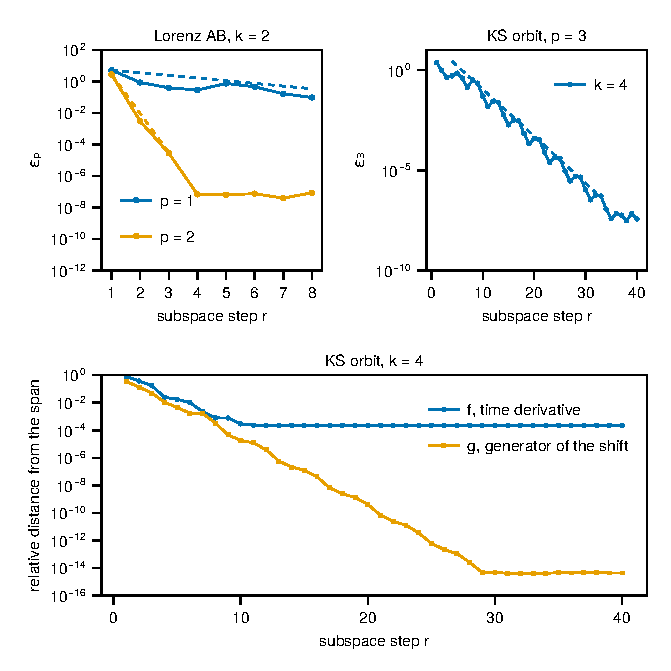
\includegraphics[width=0.8\textwidth]{figures/subspace.pdf}
  \caption{The subspace iteration on the two orbits. Top left, $\varepsilon_1$ and $\varepsilon_2$
  on the Lorenz orbit with $k = 2$. Top right, $\varepsilon_3$ on the Kuramoto--Sivashinsky orbit
  with $k = 4$, the same to rounding with $k = 3$ and $6$. Dashed lines have the slopes
  $-(\lambda_p - \lambda_{p+1})\tau$ predicted by \eqref{eq:rate} with $j = k = p$ from the
  multipliers of the dense monodromy. Bottom, the largest relative distance over the seeds of the
  time derivative and of the generator of the shift from the span of the bases, with $k = 4$.}
  \label{fig:subspacedata}
\end{figure}

With $p = 3$ the measure follows the unstable and the two neutral directions
(figure~\ref{fig:subspacedata}, top right). It falls at the rate set by the fourth multiplier,
about a factor $0.58$ per step, close to the dashed line. With $k = 3$, $4$ and $6$ from the same
random start the values agree to rounding, since without a projection step the directions beyond
the third do not act on the first three (section~\ref{sec:accuracy}). After 40 steps it is near
$10^{-8}$ and still falling.

The bottom panel tells the two neutral directions apart. The generator of the shift enters the
span of the bases down to rounding, since the shift commutes exactly with the truncated scheme.
The time derivative stops at a relative distance of about $2 \times 10^{-4}$, although the
multiplier of the time direction is one to rounding. The neutral direction of the discrete loop is
thus close to $f$ but not equal to it, by an amount of the order of the error of the time step,
which is also the error of the column of the period in the Jacobian. For this reason the test
checks the generator, and not the time derivative, against the span of the bases.

\section{Closing remarks}

The package now holds the residual of multiple shooting, its exact matrix-free Jacobian, up to the
column of the period, the sensitivity of an orbit to a parameter, and a subspace iteration with
Lust's measure of accuracy but without his projection step, all built on a few functions of a
propagator that acts on batches of states. Each piece treats the $m$ segments at
once, and the subspace iteration pays for this with time integrated, as section
\ref{sec:subspace} discusses. The bases are the natural input of a preconditioner that acts on the
unstable and neutral directions of the loop, which we leave for future work.

\bibliographystyle{plainnat}
\bibliography{refs}

\end{document}
